\documentclass[a4paper]{report}

%====================== PACKAGES ======================

\usepackage[french]{babel}
\usepackage[utf8]{inputenc}
%pour gérer les positionnement d'images
\usepackage{float}
\usepackage{amsmath}
\usepackage{graphicx}
\usepackage[colorinlistoftodos]{todonotes}
\usepackage{url}
%pour les informations sur un document compilé en PDF et les liens externes / internes
\usepackage{hyperref}
\usepackage[final]{pdfpages}
%espacement entre les lignes
\usepackage{setspace}
%modifier la mise en page de l'abstract
\usepackage{abstract}
%police et mise en page (marges) du document
\usepackage[T1]{fontenc}
\usepackage[top=2cm, bottom=2cm, left=2cm, right=2cm]{geometry}
%Pour les galerie d'images
\usepackage{subfig}

%====================== INFORMATION ET REGLES ======================

%rajouter les numérotation pour les \paragraphe et \subparagraphe
\setcounter{secnumdepth}{4}
\setcounter{tocdepth}{4}

%======================== DEBUT DU DOCUMENT ========================

\begin{document}
\begin{spacing}{2}
\newcommand{\HRule}{\rule{\linewidth}{0.5mm}}
\begin{titlepage}
\begin{center}

% Upper part of the page. The '~' is needed because only works if a paragraph has started.

\includegraphics[width=0.35\textwidth]{./logo}~\\[1cm]

\textsc{\LARGE École nationale supérieure d'informatique et d'analyse des systèmes}\\[1.5cm]

\textsc{\Large }\\[0.5cm]

% Title
\HRule \\[0.4cm]

{\huge \bfseries Projet Technologie Web \\
Application Web du réservation des terrains \\[0.4cm] }

\HRule \\[1.5cm]

% Author and supervisor
\begin{minipage}{0.4\textwidth}
\begin{flushleft} \large
\emph{Réalisé par:}\\
\textsc{LOUAFI Noureddine}\\
\textsc{OUMOUDID Othmane}\\
\textsc{MOUFAKKIR Zohair}\\
\end{flushleft}
\end{minipage}
\begin{minipage}{0.4\textwidth}
\begin{flushright} \large
\emph{Encadré par:} \\
Pr. \textsc{MAHMOUD\\EL HAMLAOUI}\\
\end{flushright}
\end{minipage}

\vfill

% Bottom of the page
{\large Année universitaire : 2020 - 2021}

\end{center}
\end{titlepage}

%page blanche
\newpage
\thispagestyle{empty}
~
\newpage
\thispagestyle{empty}
\tableofcontents
\thispagestyle{empty}
\listoffigures
\thispagestyle{empty}
\setcounter{page}{0}
%ne pas numéroter le sommaire

\newpage

%espacement entre les lignes d'un tableau
\renewcommand{\arraystretch}{1}

%====================== INCLUSION DES PARTIES ======================







\chapter*{Remerciements}
\addcontentsline{toc}{chapter}{Remerciements}

Avant tout développement sur ce projet, nous tenons à remercier du fond du cœur notre cher professeur monsieur EL HAMLAOUI Mahmoud qui nous a formé et accompagné  tout au long de notre travail avec beaucoup de patience et de pédagogie.

Un merci bien particulier adressé également à nos professeurs pour leurs remarques, leurs directives et l'intérêt qu'ils portent aux étudiants. Nous les remercions sincèrement pour leur suivi et leur orientation.


\chapter{Présentation du projet}
\section{Amenant}

\par 
Au cours de notre formation en tant qu'Elève Ingénieur de l'ENSIAS en 2ème année, nous sommes appelés à travailler sur un projet Java EE à travers lequel nous exploitons nos connaisances et compétences acquis durant notre formation \textbf{Développement et Ingéniere Web} afin d'aboutir à une application Web basé complètement sur Java EE bien construite. 

Avec l'accord de notre cher encadrant, nous avons choisi à travailler sur une application qui permet de faire la réservation des terrains en ligne. 

\section{Analyse de l'existant et problématique}

\par 
Le sport est considéré comme une activité indispensable pour tout le monde, hommes ou femmes, petits ou grands pour maintenir leur santé et developer leurs compétences physiques et morales. Aujourd'hui, faire du sport doit être une activité quotidienne pour tout le monde afin d'être plus productif et pour garder la santé. 

Ainsi au Maroc, le nombre d'espaces pour faire du sport n'est pas trés grand ,ce qui engendre plusieurs restrictions au gens qui souhaitent faire du sport, donc ils finissent finalement par abandonner.

Ils existent plusieurs restrictions, parmi eux la non organisations des terrains publics qui adoptent la méthode de premier arrivé premier servi, la chose qui peut donner naissance à des malentendus et des bagarres, notamment chez les jeunes.

Au sujet des centres qui adoptent des méthodes organisée, dans la plupart des cas, le client doit faire sa réservations soit par appel téléphonique, soit par se rendre au centre, et faire sa réservation sur place, et cela produit plusieurs problèmes tel que la longue distance, ou il se peut que le gérant du centre soit injoignable. 

\section{Solution proposée}

De ce qui précède, nous nous sommes aperçus que le problème de réservations des terrains est un problème serieux, et l'idée  de tirer profit du digital pour le résoudre est trés bonne. Pour cela, nous avons décidé de créer une application, qui peut être utilisée par le web, et qui permet au client la réservation des terrains en ligne.


Cette application aura principalement les objectifs suivants :


\begin{itemize}
\item La simplicité : Permettre au client de faire sa réservation en suivant les instructions simples de l'application par offrir une très bonne expérience utilisateur.  
\item La rapidité : Grâce à l'application Web, le processus du réservation va devenir trés rapide et plus comfortable en interagissant juste avec l'application. 

\end{itemize}


\chapter{Analyse et Conception}

\par
Pour réaliser l'analyse et la conception de
notre application web, nous avons utiliser le langage de modélistaion UML, c'est un langage de modélisation graphique à base de pictogrammes conçu comme une méthode normalisée de visualisation dans les domaines du développement logiciel et en conception orientée objet.

Dans ce projet, nous avons tirer profit de quelque'uns des diagramme propre à UML, tel que le diagramme de classe et le diagramme de cas d'utilisation.

\section{Diagramme de cas d’utilisations}

les diagrammes de cas d'utilisation modélisent le comportement d'un système et permettent de capturer les exigences du système. Les diagrammes de cas d'utilisation décrivent
les fonctions générales et la portée d'un système. Ces diagrammes identifient également les
interactions entre le système et ses acteurs. Les cas d'utilisation et les acteurs dans les diagrammes de cas d'utilisation décrivent ce que le système fait et comment les acteurs l'utilisent,
mais ne montrent pas comment le système fonctionne en interne.
\cleardoublepage
\begin{itemize}
\item Diagramme de cas d’utilisation :
\begin{figure}[!ht]
\begin{center}
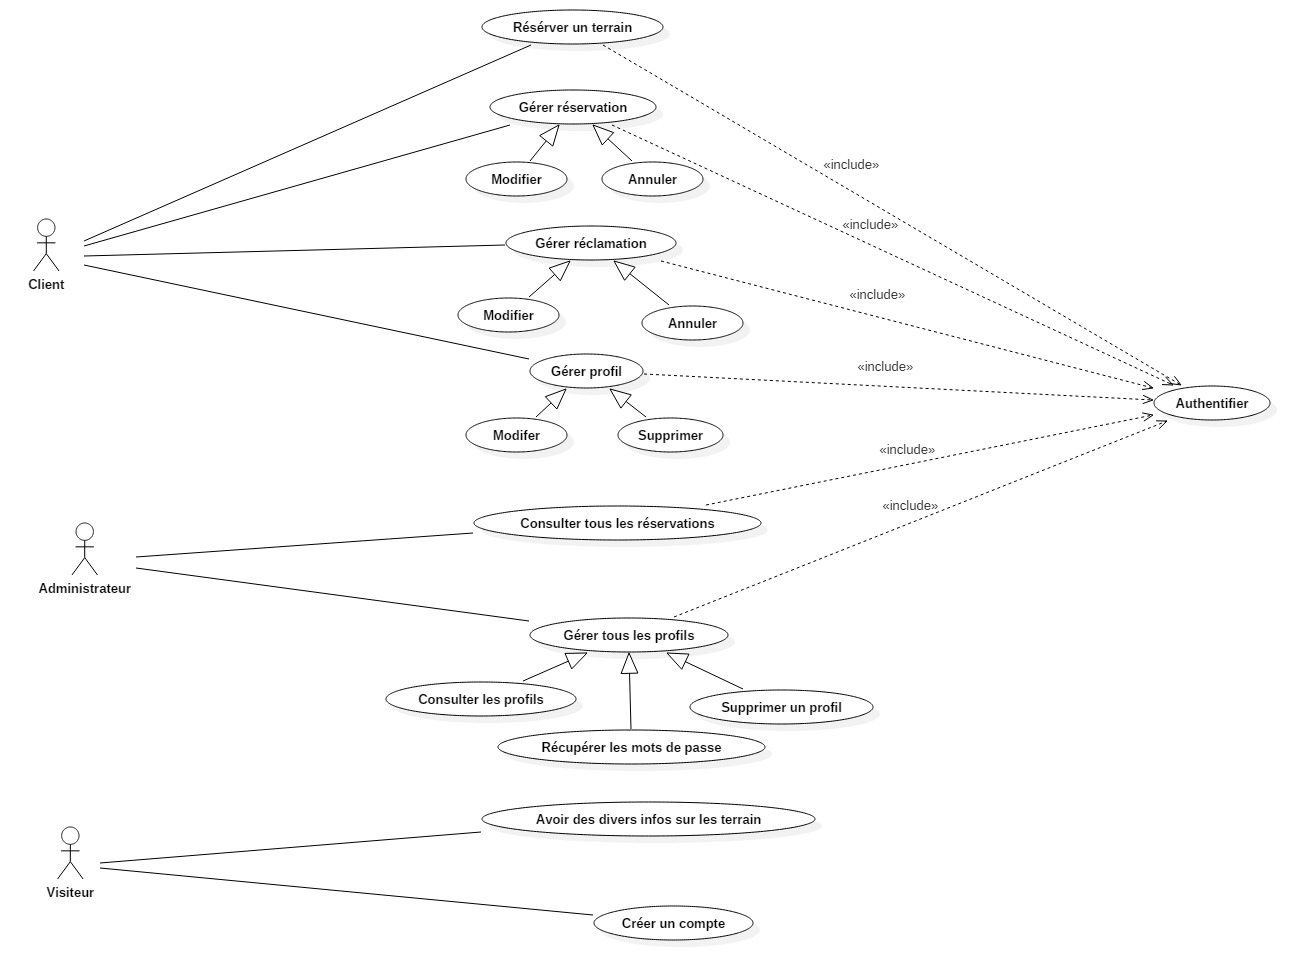
\includegraphics[height=14cm]{image/Cas_Utilisation.jpg}
\end{center}
\caption[Diagramme cas d'utilisation]{Diagramme cas d'utilisation}
\end{figure}

\cleardoublepage
 
\end{itemize}

\section{Diagramme de classe}
Le diagramme de classes est un schéma utilisé en génie logiciel pour présenter les classes et les interfaces des systèmes ainsi que leurs relations. Ce diagramme fait partie de la partie statique d'UML, ne s'intéressant pas aux aspects temporels et dynamiques.

Une classe décrit les responsabilités, le comportement et le type d'un ensemble d'objets. Les éléments de cet ensemble sont les instances de la classe.

Une classe est un ensemble de fonctions et de données (attributs) qui sont liées ensemble par un champ sémantique. Les classes sont utilisées dans la programmation orientée objet. Elles permettent de modéliser un programme et ainsi de découper une tâche complexe en plusieurs petits travaux simples.



\begin{figure}[!ht]
\begin{center}
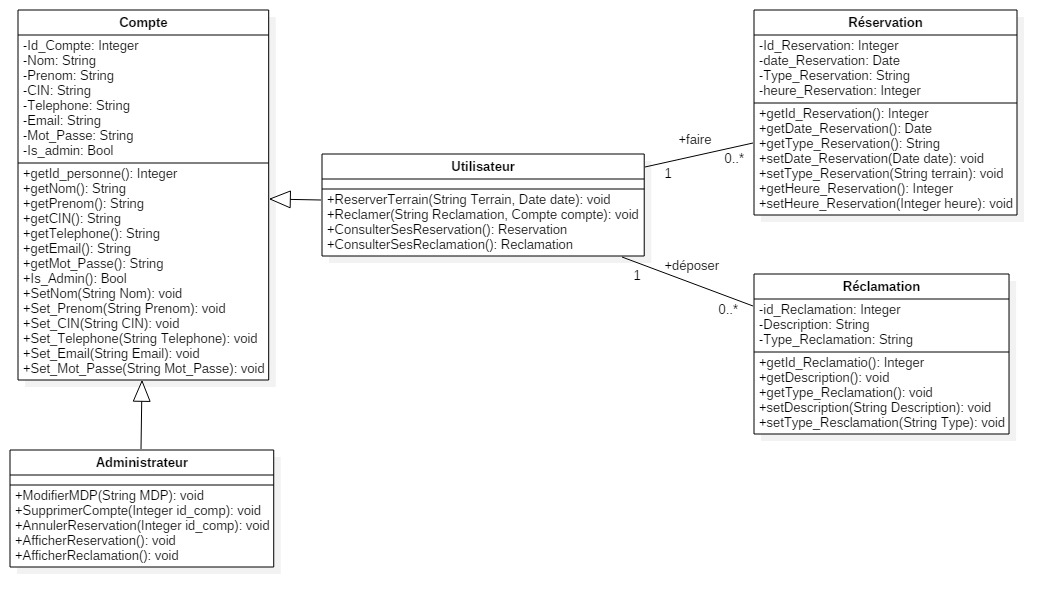
\includegraphics[height=10cm]{image/diagramme_de_classe.jpeg}
\end{center}
\caption[Diagramme de classe]{Diagramme de classe}
\end{figure}
\cleardoublepage
 


\chapter{Réalisation}
\section{les outils et les technologies}

\subsection{Pattern MVC}
Le pattern d'architecture logicielle MVC (\textbf{M}odèle-\textbf{V}ue-\textbf{C}ontrôleur) est un modèle destiné à répondre aux besoins des applications interactives en séparant les problématiques liées aux différents composants au sein de leur architecture respective..
Ce paradigme regroupe les fonctions nécessaires en trois catégories :\\
\begin{itemize}
\item[•] Un modèle : modèle de données.
\item[•] Une vue : interface utilisateur.
\item[•] Un contrôleur : logique de contrôle.\vspace{0.1cm}\\
\end{itemize}

\begin{minipage}{\linewidth}
	\makebox[\linewidth]{
		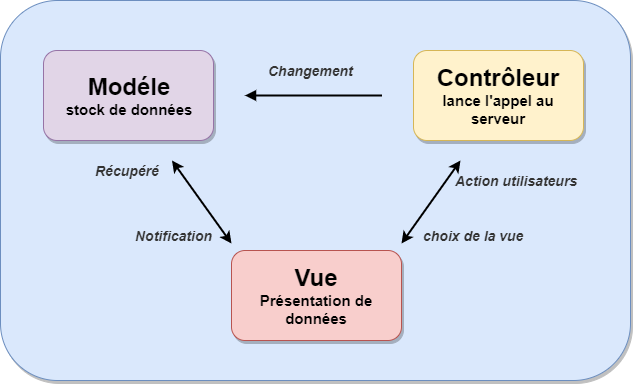
\includegraphics[keepaspectratio=true,scale=0.45]{image/mvc10}}
	\captionof{figure}{Pattern MVC.}\label{f3}%    
\end{minipage}\\
\cleardoublepage
Nous avons un premier découpage de l’application qui nous permet déjà de répondre à certaines de nos problématiques. En identifiant clairement les parties logiques, nous pouvons plus facilement maintenir notre application et la tester.\\
Voici les différents packages que nous avons utilisés pour appliquer le modèle MVC sur ce système:\\

\textbf{Package Controller:}\\
Le package Contrôleur gère la dynamique de l'application. Elle fait le lien entre l'utilisateur et le reste de l'application.\\

\textbf{Package Model:}\\
Le packege Modèle d'une architecture MVC encapsule le logique métier  ainsi que l'accès aux données. Il peut s'agir d'un ensemble de fonctions (Modèle procédural) ou de classes (Modèle orienté objet).\\

\textbf{Package View:}\\
Le packege Vue s'occupe des interactions avec l'utilisateur : présentation, saisie et validation des données\\



\subsection{Outils de développement }
\subsubsection{Langage de programmation}
\begin{minipage}{0.18\textwidth}
	\begin{minipage}{\linewidth}
	\makebox[\linewidth]{
		
\includegraphics[keepaspectratio=true,scale=0.4]{image/jee}}   
\end{minipage}
\end{minipage}
\hfill
\begin{minipage}{0.75\textwidth}
(Java Entreprise Edition) est la version entreprise de la plate-forme "Java" qui se compose de l'environnement "JSE" ainsi que de nombreuses API et composants destinés à une utilisation "côté serveur" au sein du système d'information de l'entreprise.\\
\textbf{\textit{Justification:}} JAVA est sécurisée, il a été conçu pour être exploité dans des environnements serveur et distribués. Dans ce cadre, la sécurité n’a pas été négligeable. C’est le langage le plus adopté par les développeurs grâce à sa fiabilité et sa performance élevé. \\
\end{minipage}\\

\subsubsection{Environnement de  développement}
\begin{minipage}{0.2\textwidth}
	\begin{minipage}{\linewidth}
		\makebox[\linewidth]{
			
\includegraphics[keepaspectratio=true,scale=0.06]{image/eclipse.jpg}}   
	\end{minipage}
\end{minipage}
\hfill
\begin{minipage}{0.75\textwidth}
	Eclipse est un projet, décliné et organisé en un ensemble de sous-projets de développements logiciels, de la fondation Eclipse visant à développer un environnement de production de logiciels libre qui soit extensible, universel et polyvalent, en s'appuyant principalement sur Java.

    Son objectif est de produire et fournir des outils pour la réalisation de logiciels, englobant les activités de programmation (notamment environnement de développement intégré et frameworks) mais aussi d'AGL recouvrant modélisation, conception, test, gestion de configuration, reporting… Son EDI, partie intégrante du projet, vise notamment à supporter tout langage de programmation à l'instar de Microsoft Visual Studio.
\end{minipage}\\
\subsubsection{Gestion de version \& collaboration:}
\begin{minipage}{0.2\textwidth}
	\begin{minipage}{\linewidth}
		\makebox[\linewidth]{
			
\includegraphics[keepaspectratio=true,scale=0.12]{image/git}}   
	\end{minipage}
\end{minipage}
\hfill
\begin{minipage}{0.75\textwidth}
	Git est un logiciel de gestion de versions décentralisé. C'est un logiciel libre créé par Linus Torvald, auteur du noyau Linux, et distribué selon les termes de la licence publique générale GNU version 2. En 2016, il s’agit du logiciel de gestion de versions le plus populaire qui est utilisé par plus de douze millions de personnes.\\
\end{minipage}\\

\begin{minipage}{0.2\textwidth}
	\begin{minipage}{\linewidth}
		\makebox[\linewidth]{
			
\includegraphics[keepaspectratio=true,scale=0.04]{image/github}}   
	\end{minipage}
\end{minipage}
\hfill
\begin{minipage}{0.75\textwidth}
GitHub est un service web d'hébergement et de gestion de développement de logiciels, utilisant le logiciel de gestion de versions Git. Ce site est développé en Ruby on Rails et Erlang par Chris Wanstrath, PJ Hyett et Tom Preston-Werner. GitHub propose des comptes professionnels payants, ainsi que des comptes gratuits pour les projets de logiciels libres. Le site assure également un contrôle d'accès et des fonctionnalités destinées à la collaboration comme le suivi des bugs, les demandes de fonctionnalités, la gestion de tâches et un wiki pour chaque projet.\\
\end{minipage}\\

\subsubsection{Design \& Multimédia:}
\begin{minipage}{0.2\textwidth}
	\begin{minipage}{\linewidth}
		\makebox[\linewidth]{
			
\includegraphics[keepaspectratio=true,scale=0.3]{image/html}}   
	\end{minipage}
\end{minipage}
\hfill
\begin{minipage}{0.75\textwidth}
	L'HyperText Markup Language, généralement abrégé HTML, est le langage de balisage conçu pour représenter les pages web. C'est un langage permettant d'écrire de l'hypertexte, d'où son nom.\\
\end{minipage}\\

\begin{minipage}{0.2\textwidth}
	\begin{minipage}{\linewidth}
		\makebox[\linewidth]{
			
\includegraphics[keepaspectratio=true,scale=0.04]{image/css}}   
	\end{minipage}
\end{minipage}
\hfill
\begin{minipage}{0.75\textwidth}
	Les feuilles de style en cascade, généralement appelées CSS de l'anglais Cascading Style Sheets, forment un langage informatique qui décrit la présentation des documents HTML et XML. Les standards définissant CSS sont publiés par le World Wide Web Consortium.\\
\end{minipage}\\
\begin{minipage}{0.28\textwidth}
	\begin{minipage}{\linewidth}
		\makebox[\linewidth]{
			
\includegraphics[keepaspectratio=true,scale=0.31]{image/js}}   
	\end{minipage}
\end{minipage}
\hfill
\begin{minipage}{0.75\textwidth}
	JavaScript (qui est souvent abrégé en « JS ») est un langage de script léger, orienté objet, principalement connu comme le langage de script des pages web.\\
\end{minipage}\vspace{0.5cm}\\
\begin{minipage}{0.2\textwidth}
	\begin{minipage}{\linewidth}
		\makebox[\linewidth]{
			
\includegraphics[keepaspectratio=true,scale=0.18]{image/eee}}   
	\end{minipage}
\end{minipage}
\hfill
\begin{minipage}{0.75\textwidth}
	La JavaServer Pages Standard Tag Library est un composant de la plate-forme JEE de développement. Elle étend la spécification JSP en ajoutant une bibliothéque de balises pour les taches courantes, comme le travail sur des fichiers XML, l'exécution conditionnelle, les boucles et l'internationalisation.
\end{minipage}\vspace{0.5cm}\\
\subsubsection{Serveur d’application:}
\begin{minipage}{0.2\textwidth}
	\begin{minipage}{\linewidth}
		\makebox[\linewidth]{
			
\includegraphics[keepaspectratio=true,scale=0.31]{image/tomcat}}   
	\end{minipage}
\end{minipage}
\hfill
\begin{minipage}{0.75\textwidth}
	Tomcat est un conteneur web libre de servlets et JSP. Issu du projet Jakarta, c'est un des nombreux projets de l’Apache Software Foundation.\\
\end{minipage}\\
\section{Présentation de l'application}
Cette partie dénombre la présentation des Scénarios applicatifs de l’application. Nous allons présenter dans ce qui suit, les imprimes-écran des principales interfaces réalisées dans notre site web.
\subsection{Page d'accueil}
C’est la page d’accueil qui s’affiche dès l’accès à notre site web, elle est constituer de trois parties principales :\\
$\bullet$ Un slider animé qui affiche les photos des différents térrains que l'application gére.\\
$\bullet$ Services: Une partie qui donne divers informations sur les les terrains qu'on possède.\\
$\bullet$ Une partie qui permet de contacter les administrateurs, ainsi qu'une carte "Google Maps", qu'affiche la localisation des terrains.\\ 
\begin{figure}[!ht]
\begin{center}
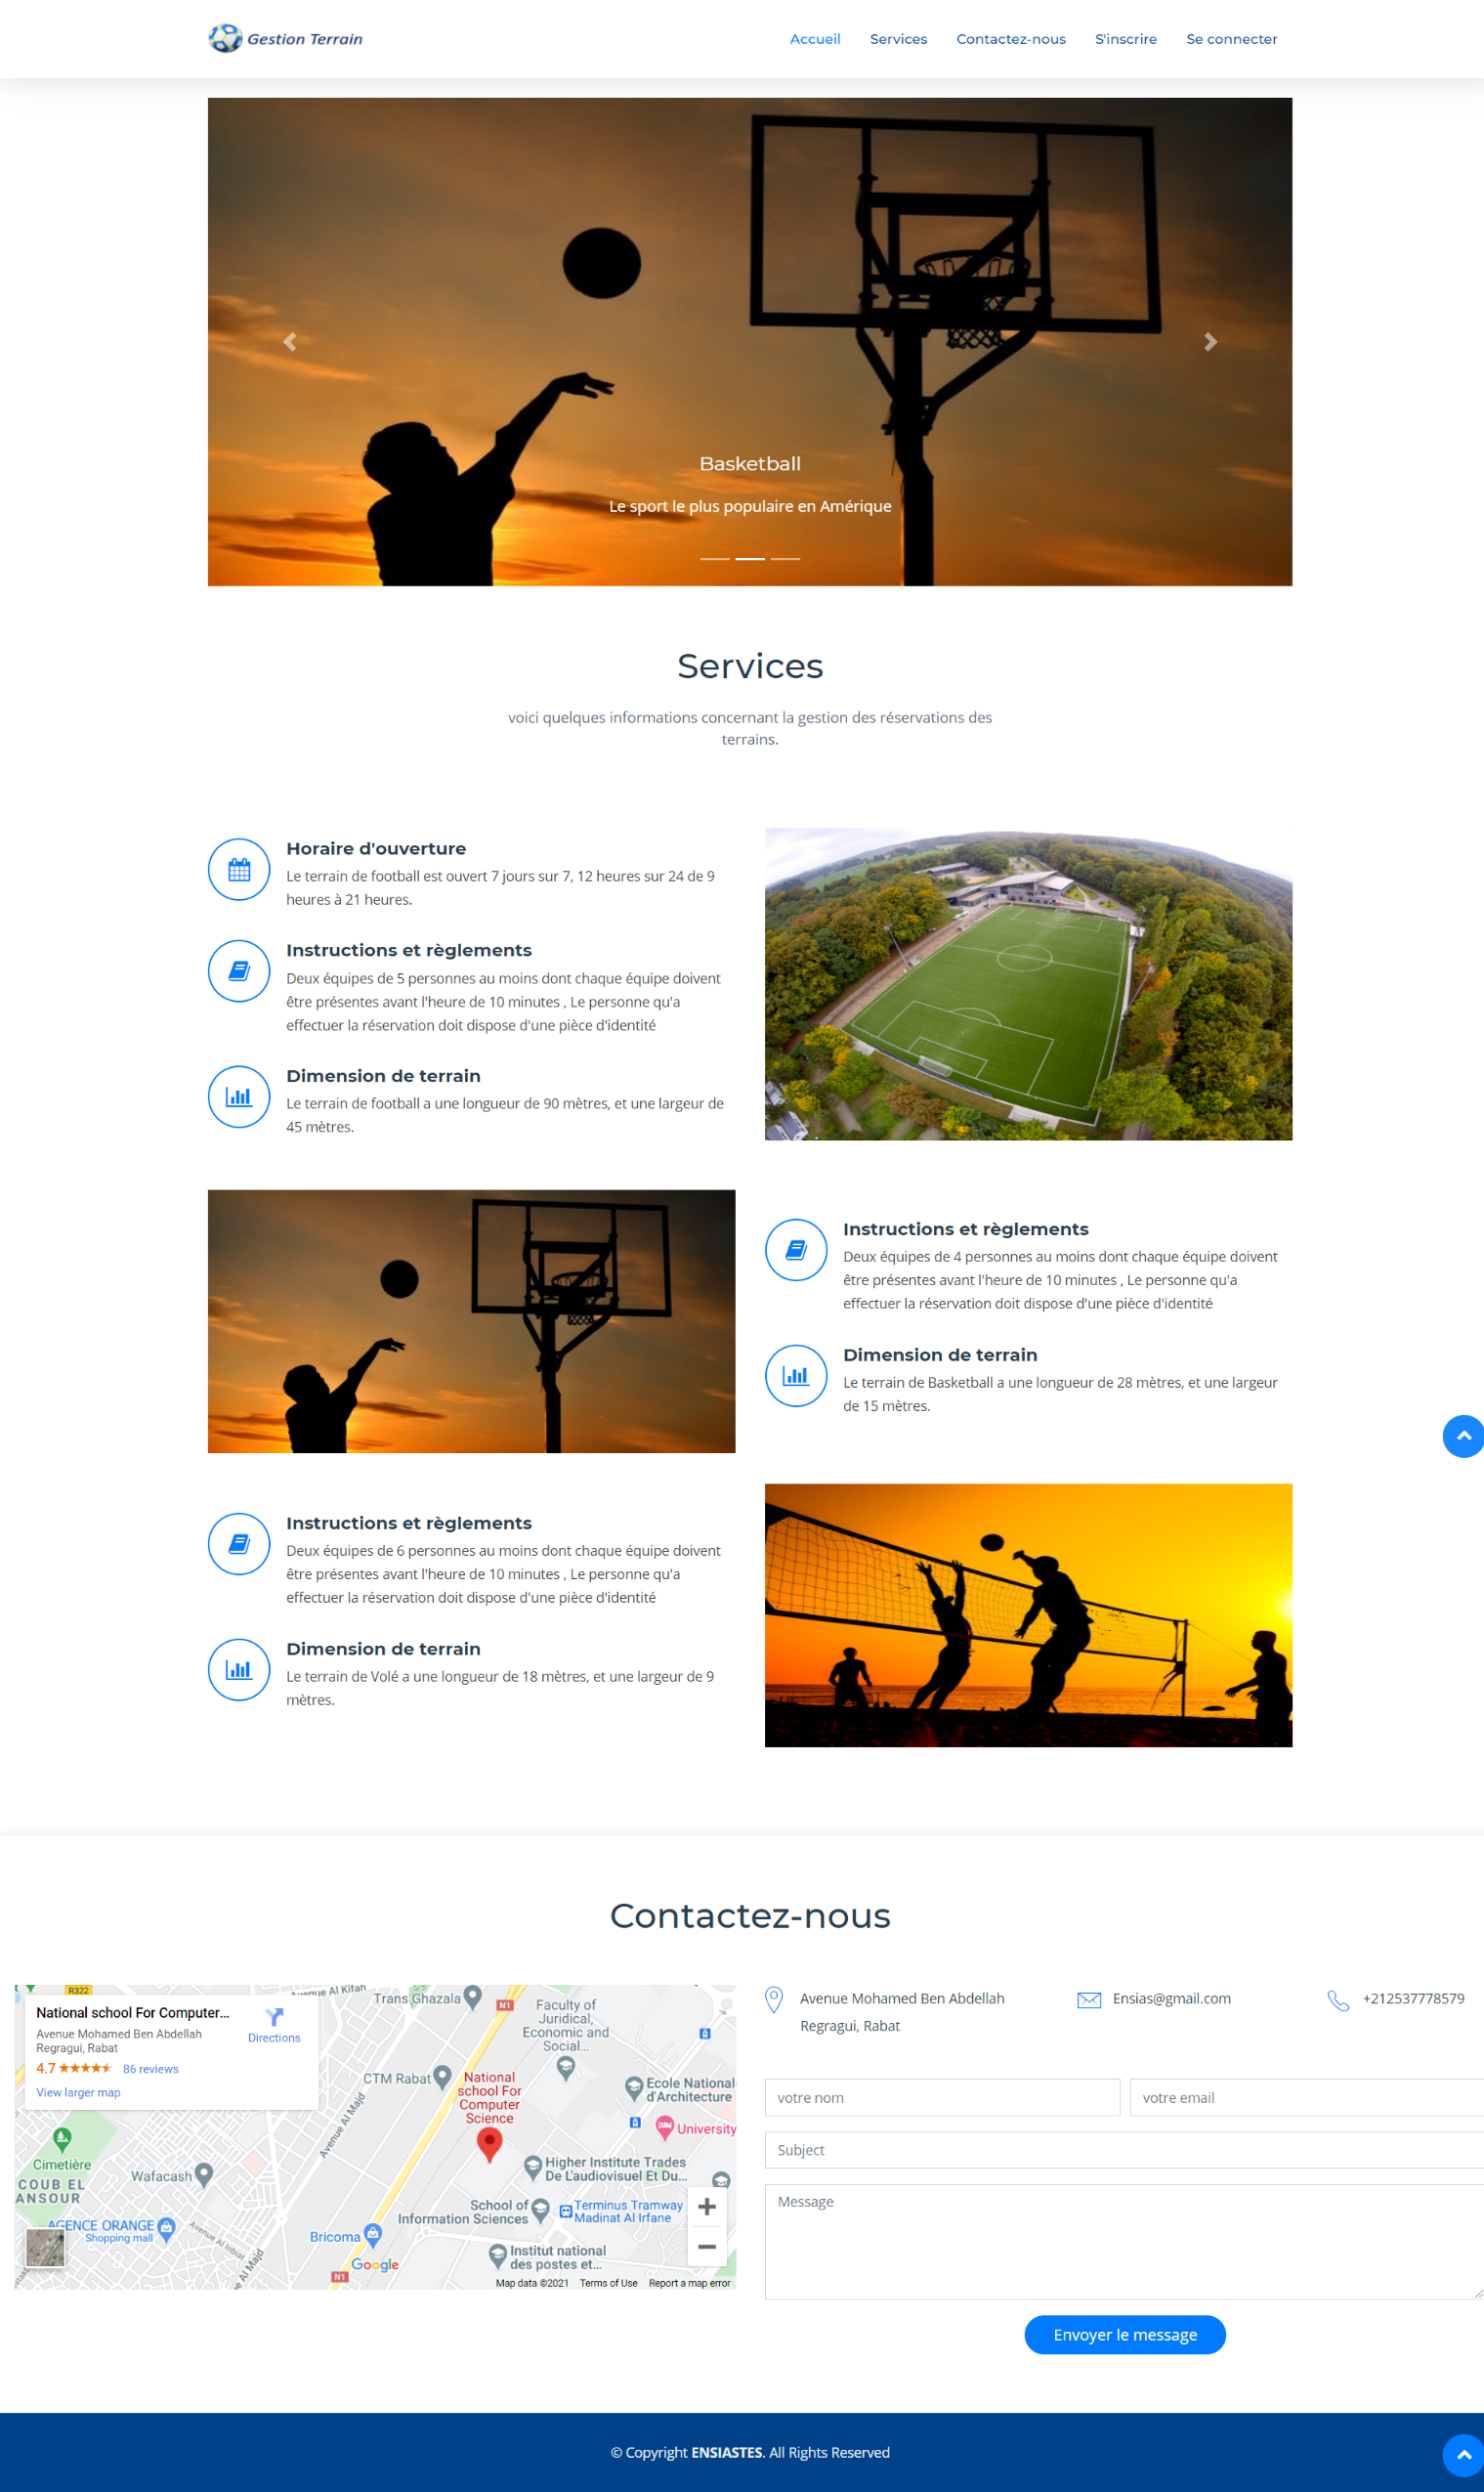
\includegraphics[width=14cm]{Screenshots/Acceuil.png}
\end{center}
\caption[Page d'accueil]{Page d'accueil}
\end{figure}

\cleardoublepage


\subsection{Page d'authentification}
Pour bénéficier de cette platforme, le client doit obligatoirement s'identifier pour pouvoir stocker ses données, s'il ne posséde pas un compte, il peut le créer rapidement en remplissant le formulaire d'inscription.\\ 
\begin{figure}[!ht]
\begin{center}
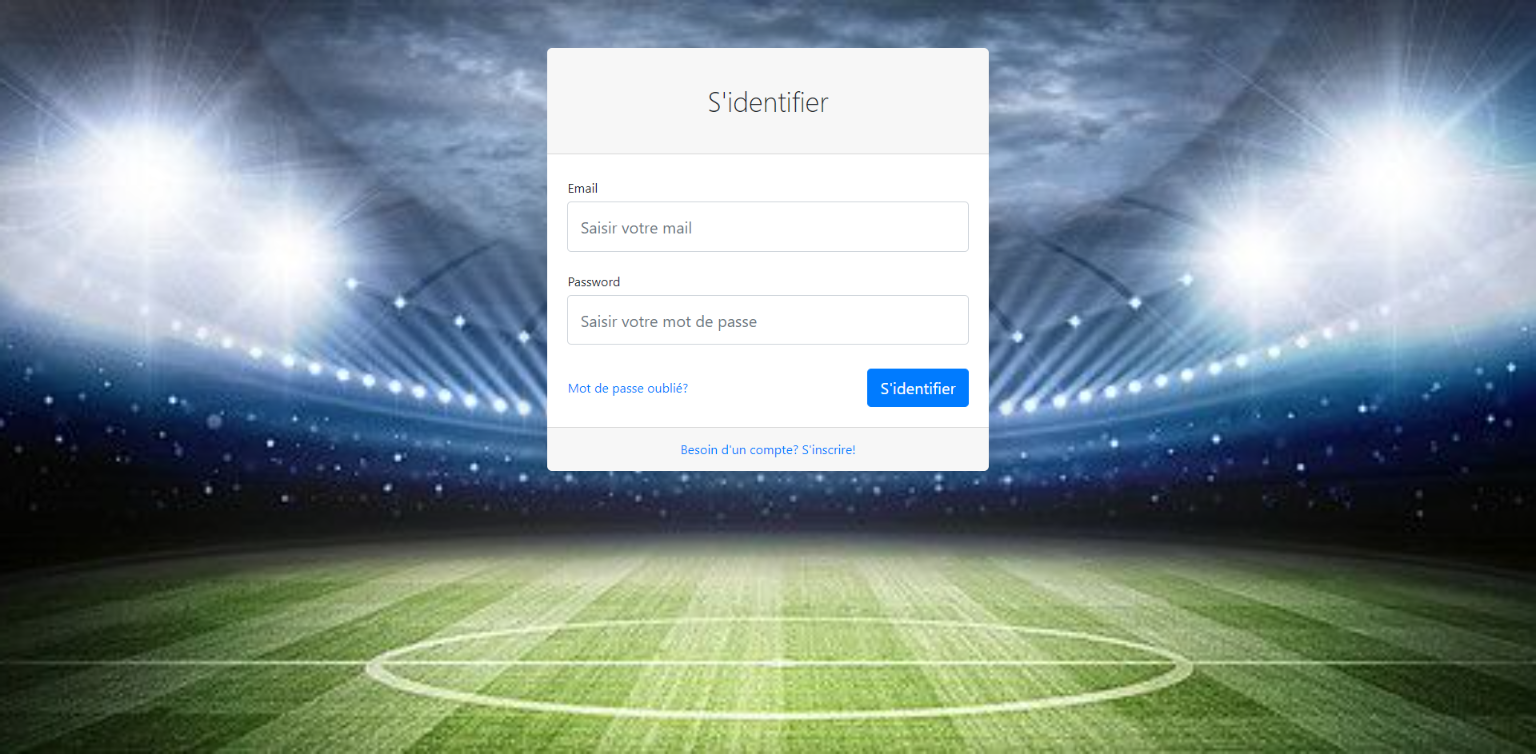
\includegraphics[width=18cm]{Screenshots/S'identifier.png}
\end{center}
\caption[Page d'identification]{Page d'identification}
\end{figure}

\begin{figure}[!ht]
\begin{center}
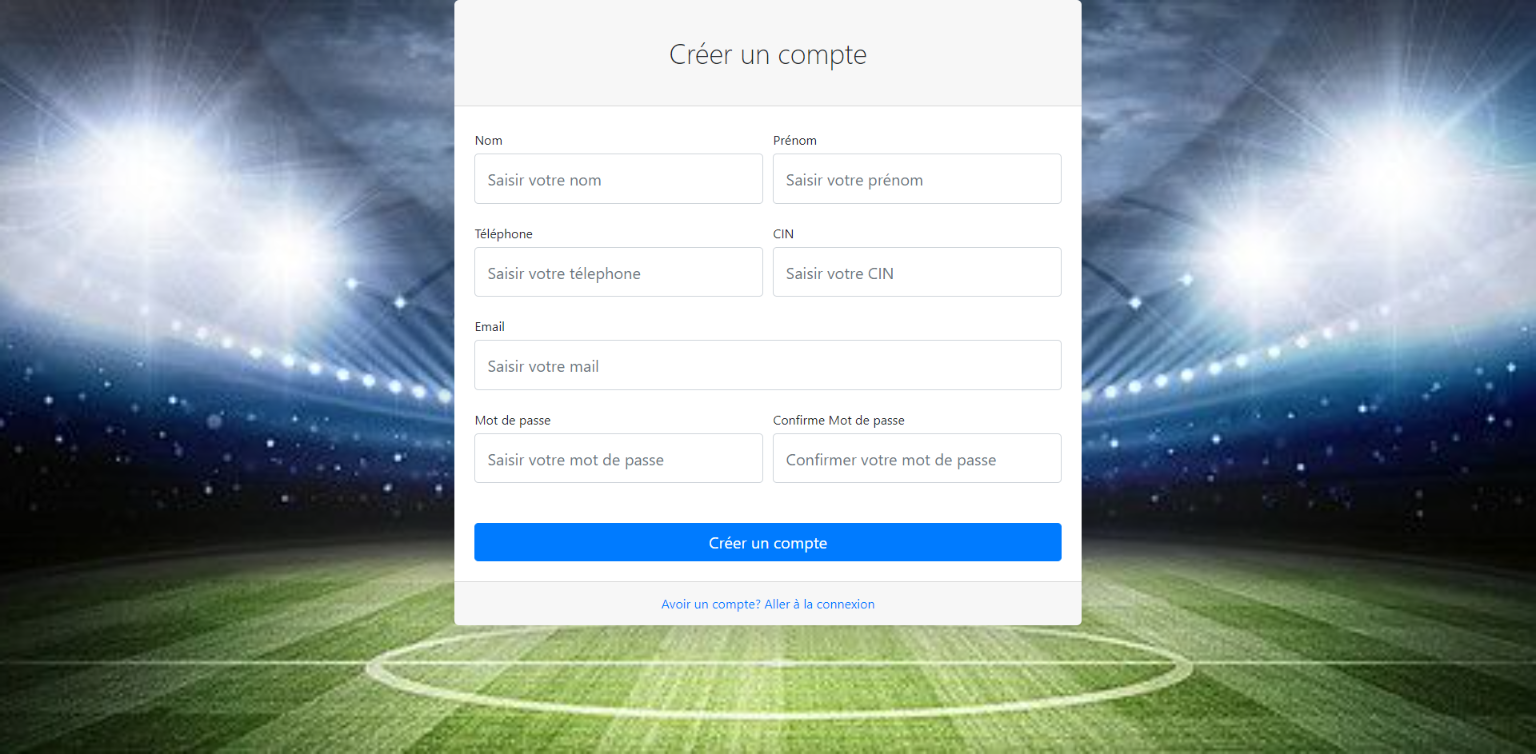
\includegraphics[width=18cm]{Screenshots/CreerCompte.png}
\end{center}
\caption[Page d'inscription]{Page d'inscription}
\end{figure}



\subsection{Espace Client}
Dans cette section, nous allons présenter tous les fonctionnalités que cette application fournit aux clients.
\subsubsection{Ajout d'une résérvation}
Pour faire une réservation, le client doit, dans un premier temps, choisir le type de terrain, puis effectuer la réservation en consultant un tableau qui affichent les horraires disponibles  tout au long de la semaine. 
, dans une limite d'une réservation par jour, et 5 par mois.
\begin{figure}[!ht]
\begin{center}
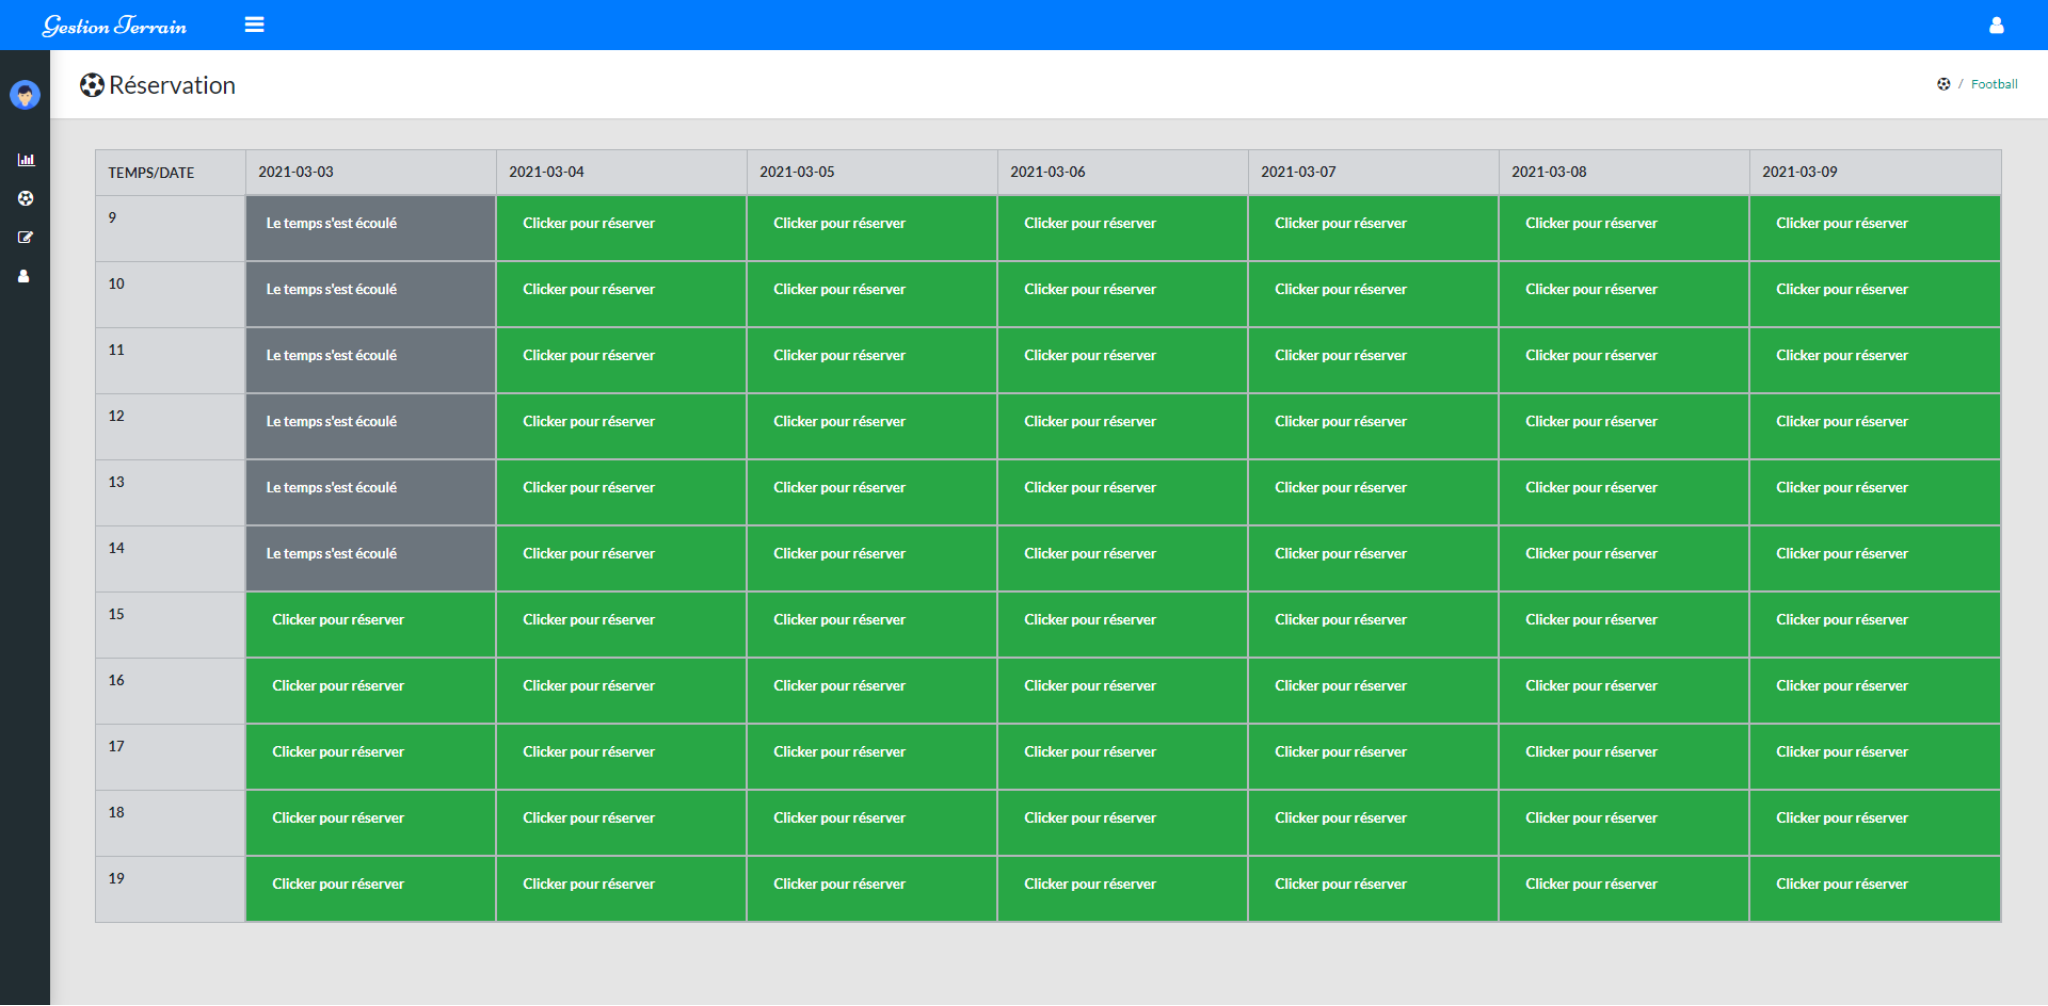
\includegraphics[width=18cm,height=12cm]{Screenshots/Reservation-Client.png}
\end{center}
\caption[Tableau de réservation]{Tableau de réservation}
\end{figure}

\subsubsection{Ajouter d'une réclamation}
Pour ajouter une réclamation, Le client doit remplir un formulaire qui contient deux champs, un champs pour pour le type de terrain, et un autre pour le corps de message de réclamation.
Le client peut également consulter la liste de toutes les réclamations qui a créé.
\cleardoublepage


\begin{figure}[!ht]
\begin{center}
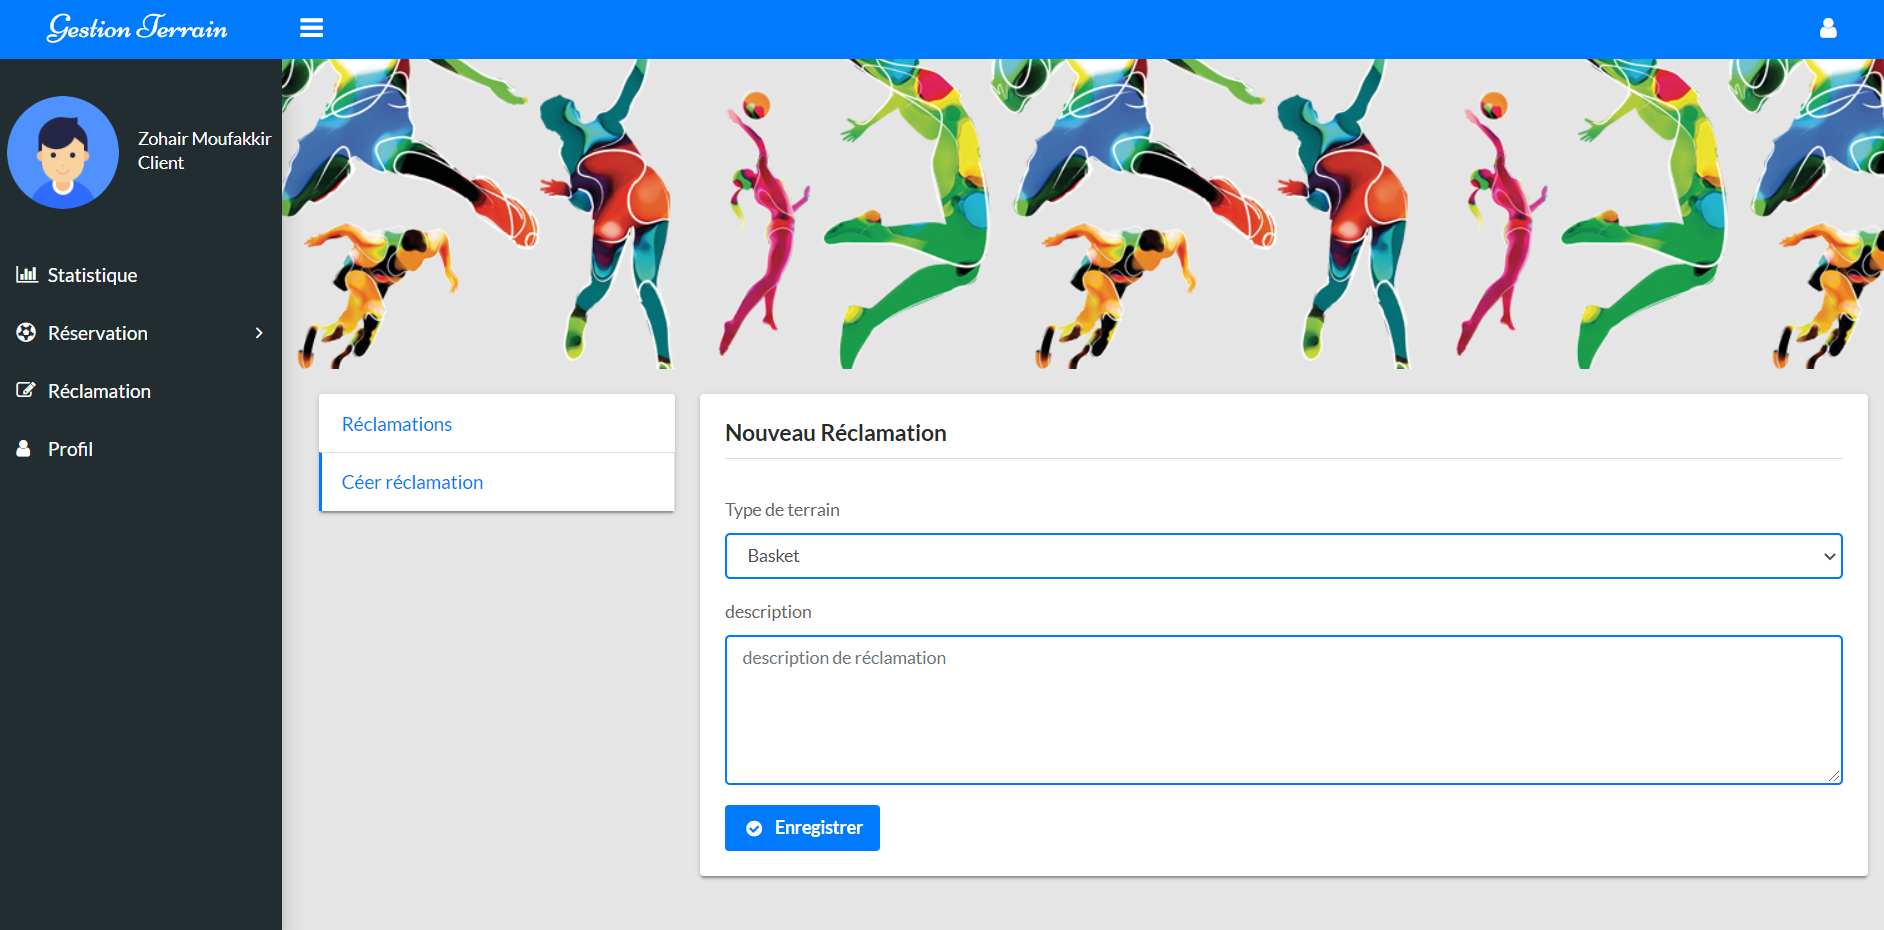
\includegraphics[width=18cm]{Screenshots/Reclamation.png}
\end{center}
\caption[Ajouter réclamation]{Ajouter réclamation}
\end{figure}


\begin{figure}[!ht]
\begin{center}
\includegraphics[width=18cm]{Screenshots/réclamation-client-list.jpg}
\end{center}
\caption[Liste de réclamation]{Liste de réclamation}
\end{figure}
\cleardoublepage

\subsubsection{Profil client}
Cette page représente des informations détailler d'un compte utilisateur, elle donne ainsi la possibilité de changer les informations personnelles de l'utilisateur et de consulter quelques statistiques de réservation et de réclamation.

\begin{figure}[!ht]
\begin{center}
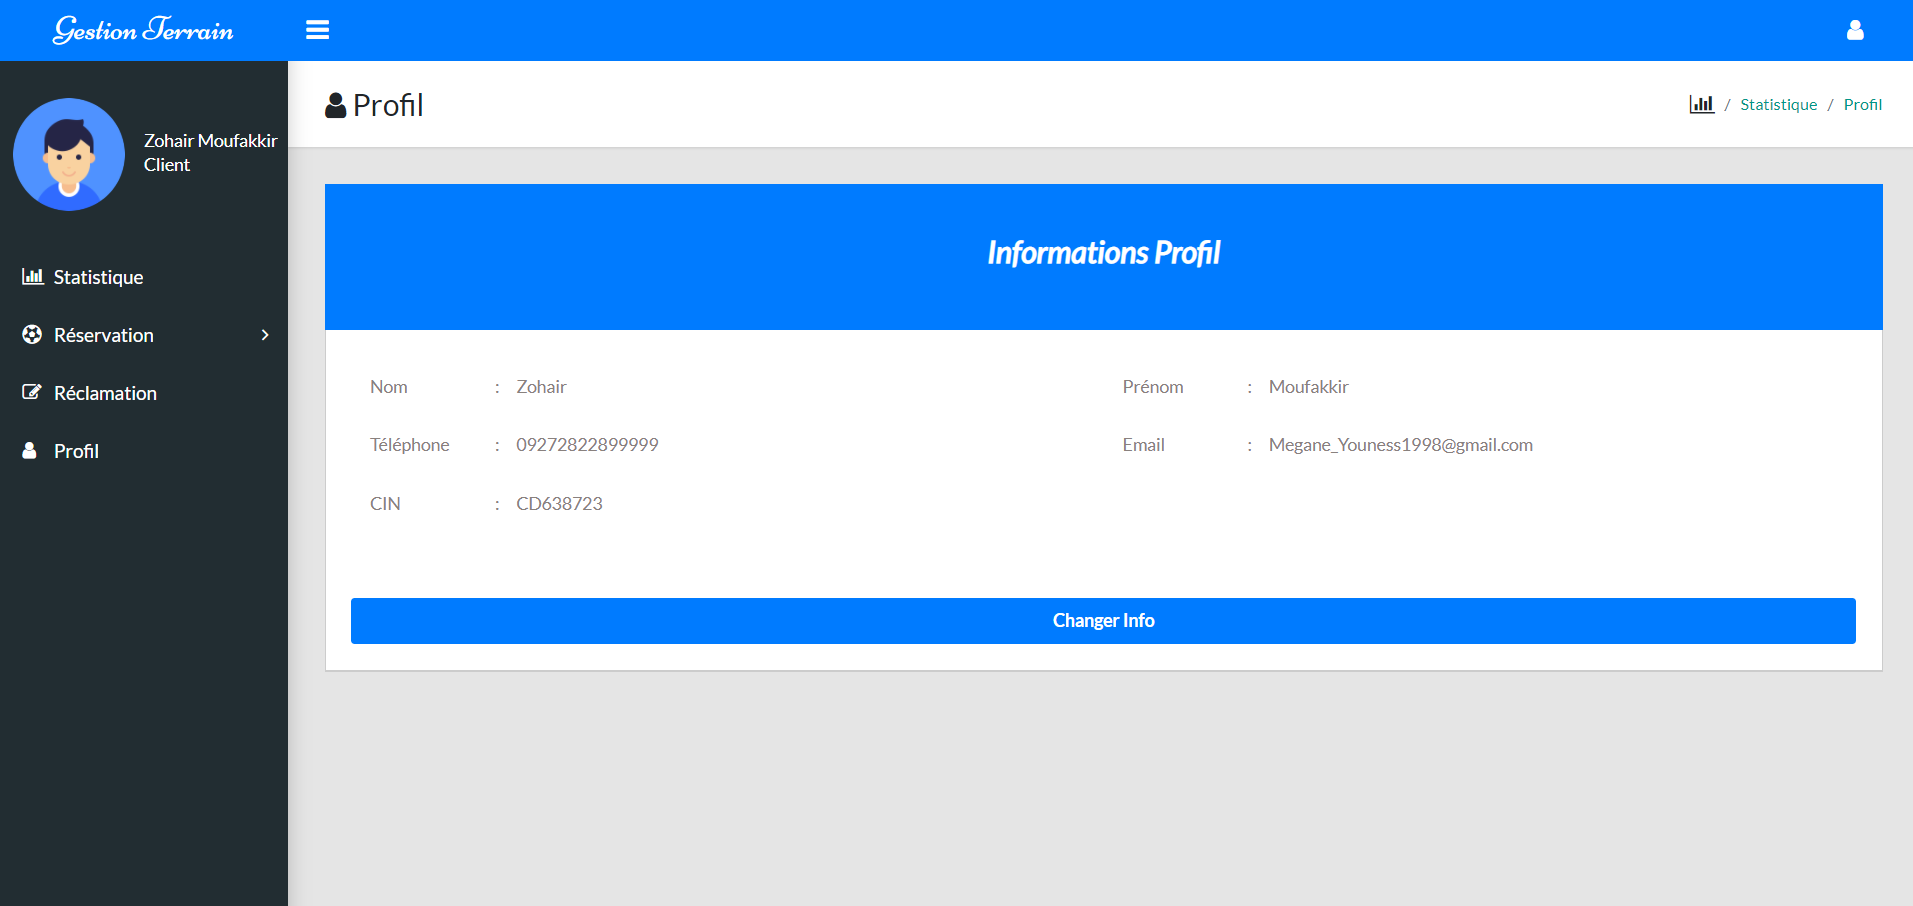
\includegraphics[width=18cm]{Screenshots/Profil-Client.png}
\end{center}
\caption[Profil du client]{Profil du client}
\end{figure}

\begin{figure}[!ht]
\begin{center}
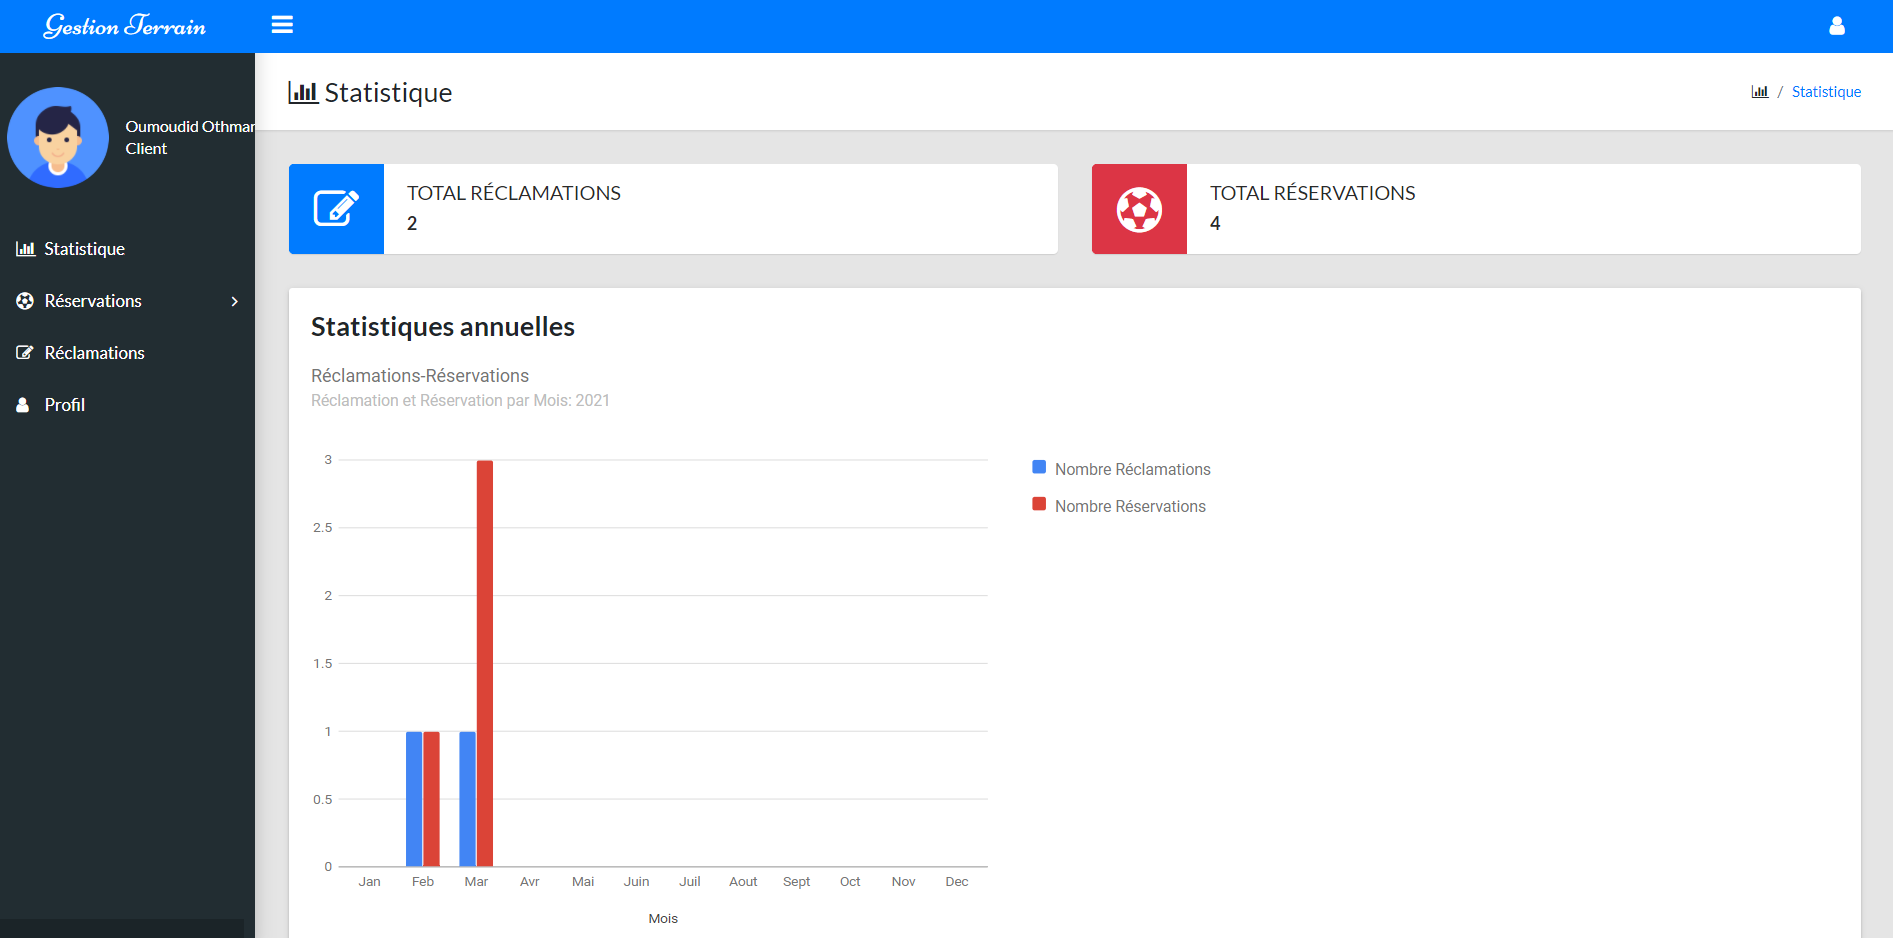
\includegraphics[width=18cm]{Screenshots/stats-clients.jpg}
\end{center}
\caption[Statistiques du client]{Statistiques du client}
\end{figure}


\subsection{Espace admin}
Cette section va mettre en évidence tous les opération que l'administrateur peut faire afin de controller l'application, et afin de rendre l'administration efficace.
\subsubsection{Consulter tous les résérvations}
L'administrateur peut consulter la liste de toutes les réservation, cette liste est munié d'informations confidentielle de chaque client. 

\begin{figure}[!ht]
\begin{center}
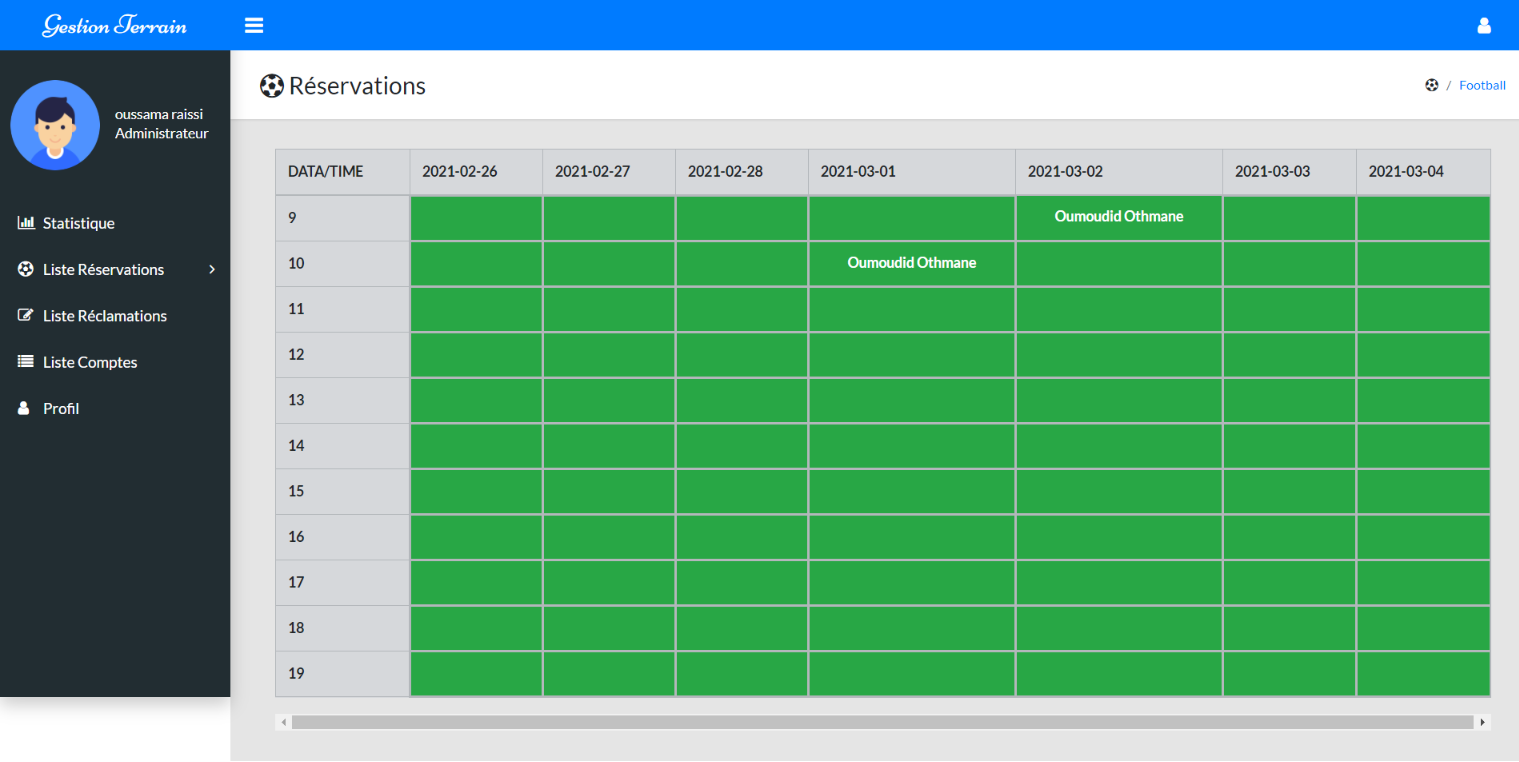
\includegraphics[width=16cm]{Screenshots/ConsulterReserv.png}
\end{center}
\caption[Toute les réservations]{Toute les réservations}
\end{figure}

\begin{figure}[!ht]
\begin{center}
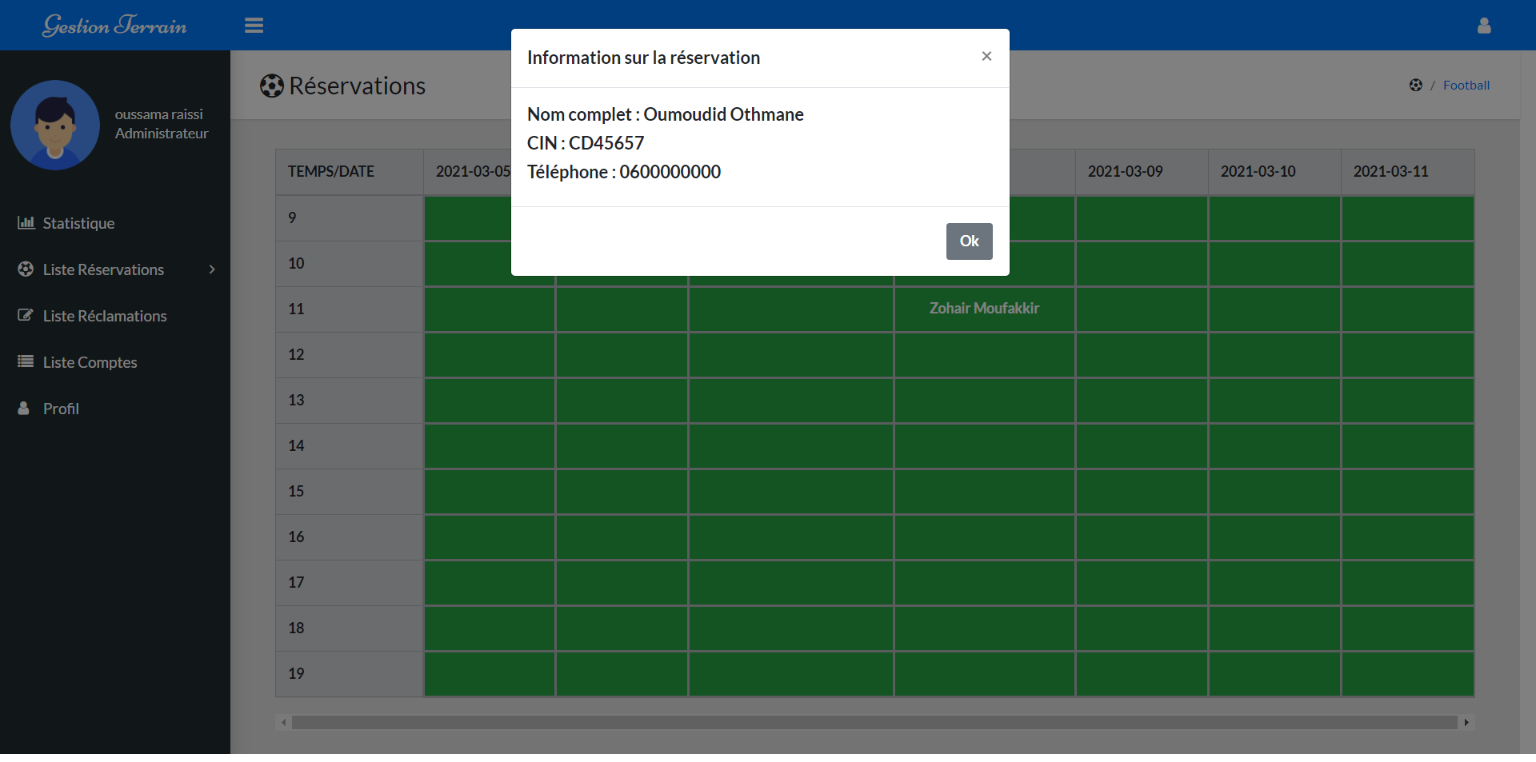
\includegraphics[width=16cm]{Screenshots/Information-reservations.png}
\end{center}
\caption[Informations confidentielles]{Informations confidentielles }
\end{figure}


\subsubsection{Consulter tous les réclamations}
L'administrateur peut consulter la liste de tous les réclamations qui ont été déja créé par les clients.
\begin{figure}[!ht]
\begin{center}
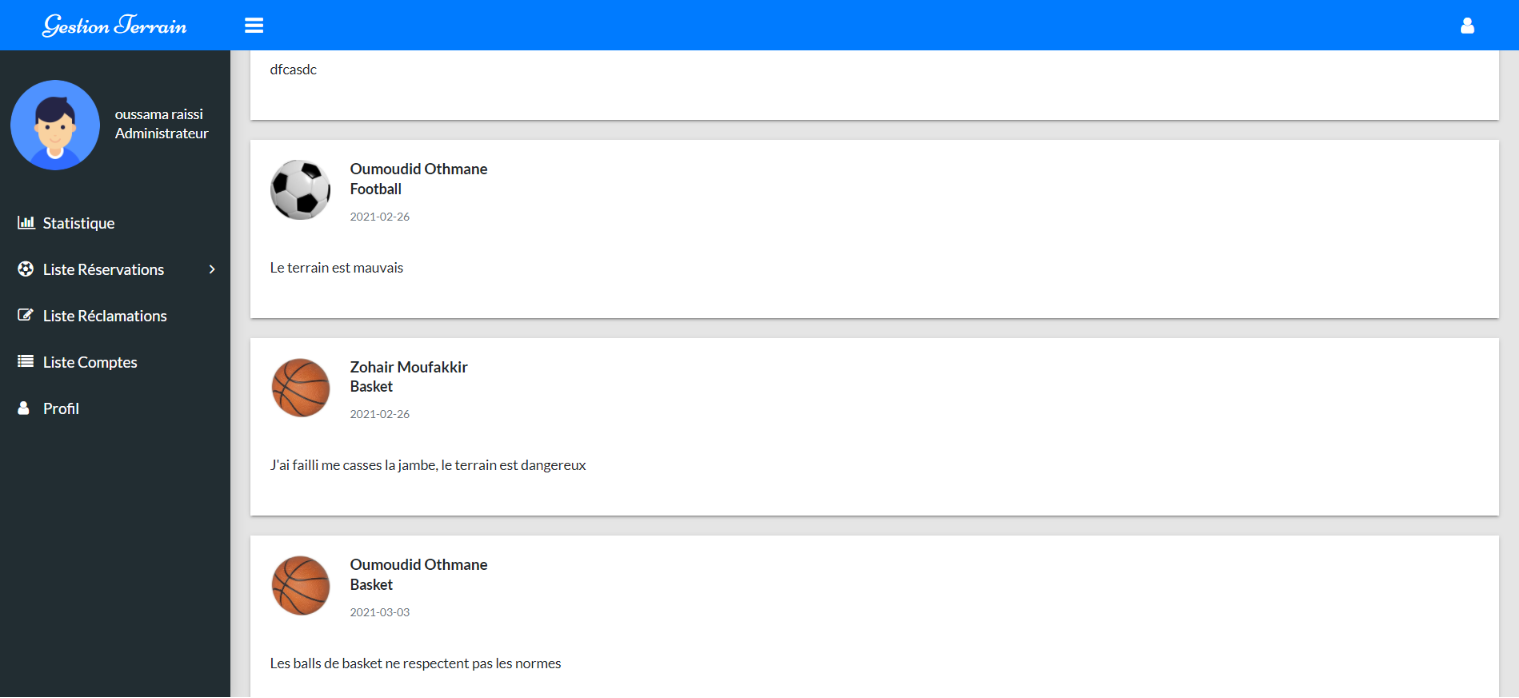
\includegraphics[width=18cm]{Screenshots/all-Reclam.png}
\end{center}
\caption[Liste des réclamations]{Liste des réclamations}
\end{figure}
\subsubsection{Consulter tous les comptes}
L'administrateur peut aussi consulter la liste de tous les clients avec la possibilté de supprimer des comptes, et de changer les mots de passes.
\begin{figure}[!ht]
\begin{center}
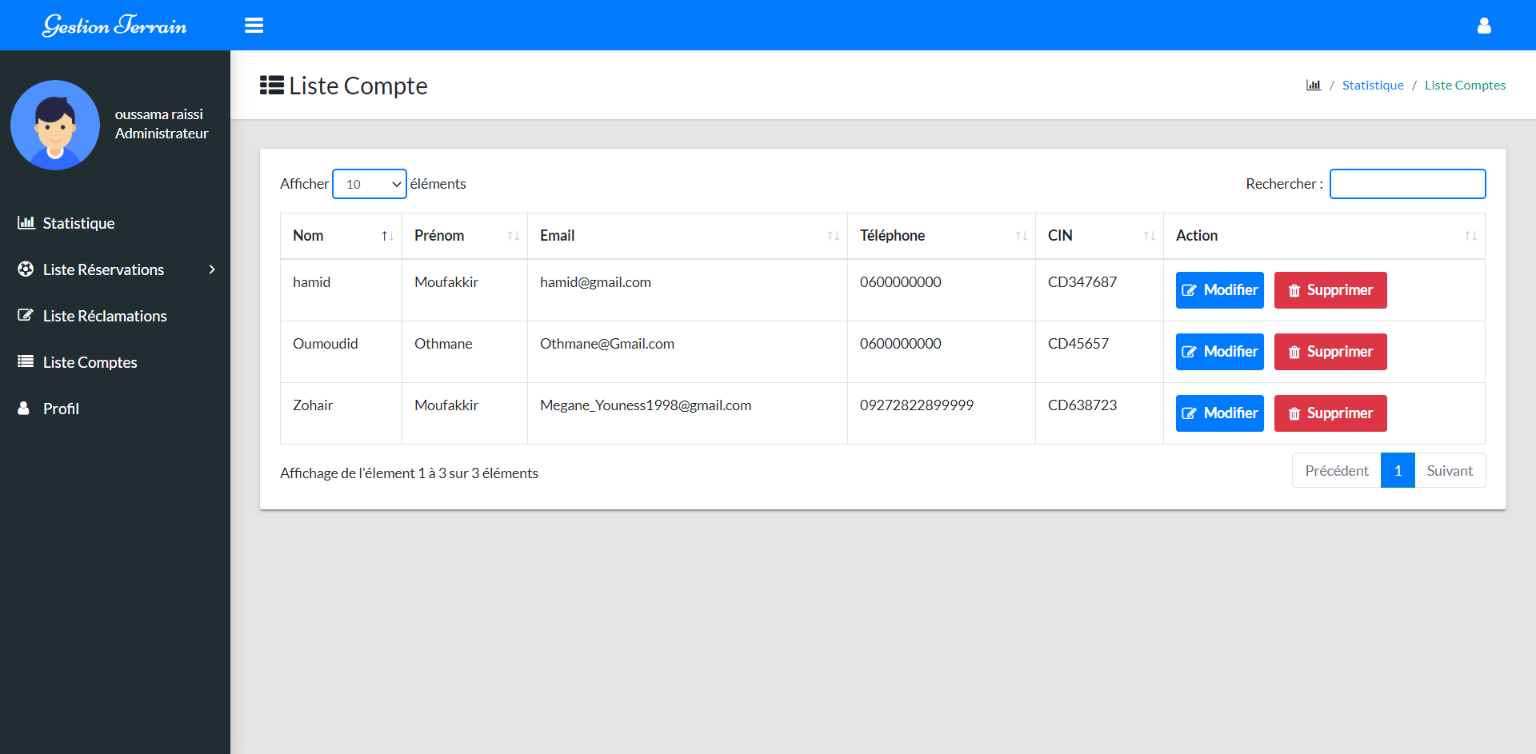
\includegraphics[width=18cm]{Screenshots/ToutLesComptes.png}
\end{center}
\caption[Liste des comptes]{Liste des Comptes}
\end{figure}


\end{spacing}

\end{document}